\documentclass{article} % For LaTeX2e
\usepackage{nips15submit_e,times}
\usepackage[colorlinks,linkcolor=red]{hyperref}
\usepackage{url}
\usepackage{amsmath}
\usepackage{graphicx}
\usepackage{float}
\usepackage{bm}
\usepackage{amssymb}
%\documentstyle[nips14submit_09,times,art10]{article} % For LaTeX 2.09


\title{CS499 Homework 1}


\author{
	Intersteller\thanks{ Use footnote for providing further information
		about author (webpage, alternative address)---\emph{not} for acknowledging
		funding agencies.}
	Department of Computer Science
	Cranberry-Lemon University
	Pittsburgh, PA 15213
}

% The \author macro works with any number of authors. There are two commands
% used to separate the names and addresses of multiple authors: \And and \AND.
%
% Using \And between authors leaves it to \LaTeX{} to determine where to break
% the lines. Using \AND forces a linebreak at that point. So, if \LaTeX{}
% puts 3 of 4 authors names on the first line, and the last on the second
% line, try using \AND instead of \And before the third author name.

\newcommand{\fix}{\marginpar{FIX}}
\newcommand{\new}{\marginpar{NEW}}

%\nipsfinalcopy % Uncomment for camera-ready version

\begin{document}
	
	
	\maketitle
	
	\section{Broken Chessboard and Jumping With Coins}
	\subsection{Tiling a Damaged Checkerboard}
	\textbf{Exercise 1.1}\par
	Color the checkerboard with black and white as the following figure.
	\begin{figure}[H]
		\centering
		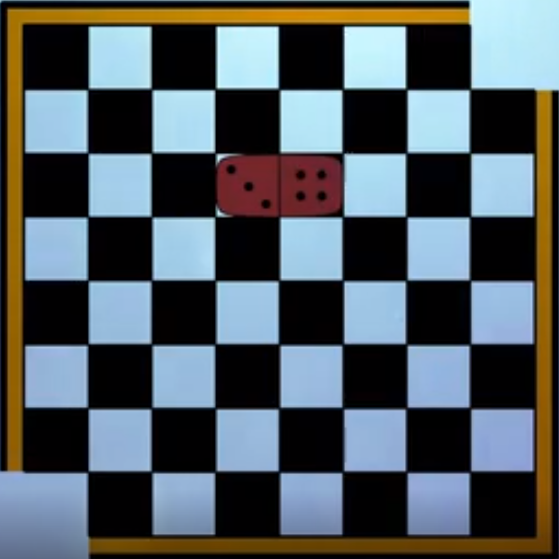
\includegraphics[scale=0.6]{1-1.png}
		\caption{}
		\label{fig:1}
	\end{figure}
	From the figure, it is obvious that one domino stone will occupy one couple of black and white grids. However, it is clear that there are 2 more black grids than white grids. Therefore, however we put the domino stones, there are always 2 black grids that can not be occupied in the end. Thus, one cannot tile the checkerboard with domino stones.\\
	
	\textbf{Exercise 1.2}\par
	Based on the previous question, we have known that it is an essential requirement that the number of yellow squares and black squares must be the same.\\
	Step 1: Let's consider the part with a red circle. In the red circle, there are 5 yellow squares and 6 black squares. So we must add a yellow square to this part in order to reach a balance. There is only one yellow square meeting the requirement, as is marked with a green circle in Fig.2.And the black square marked with star must be excluded from the red area.\\
	\begin{figure}[H]
		\centering
		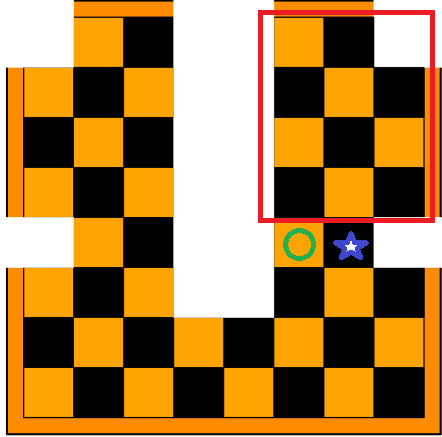
\includegraphics[scale=0.6]{f1.png}
		\caption{}
		\label{fig:2}
	\end{figure}
	
	Step 2: Based on the previous discussion, the area below the red circle can be only filled in this way, as is shown in Fig.3 . However, the two black squares marked with triangle both need the yellow square marked with circle. So there is no solution for this chessboard.
	\begin{figure}[H]
		\centering
		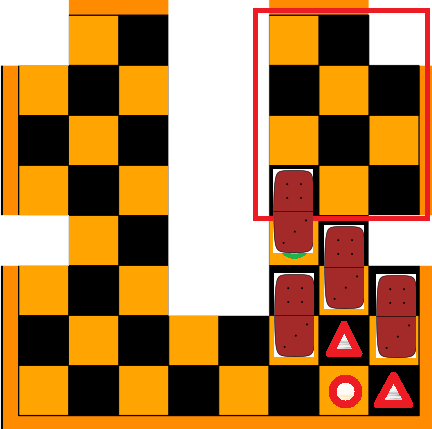
\includegraphics[scale=0.6]{f2.png}
		\caption{}
		\label{fig:3}
	\end{figure}
	
	\subsection{Jumping with Coins}
	\textbf{Exercise 1.3}\par
	Include the 2 coins into a rectangular coordinate. Assume that the first coin is in $(x_1,y_1)$ and the second in $(x_2,y_2)$. Assume the distance between the 2 coins is $L$. Now jump any one of the coins through the other one. Without loss of generality, jump the first coin. The first coin can only jump to $(2x_2-x1,2y_2-y1)$. Through simple calculation, it is clear that the current distance between the two coins is still $L$. Thus, the distance between the coins is fixed. Therfore, one cannot increase the distance between the two coins. \\
	
	\textbf{Exercise 1.4}\par
	Assume we have moved the coins to a random triangle $ABC$. Without loss of generality, we move the coin $A$ to $A'$, as in the following figure.
	\begin{figure}[H]
	\centering
	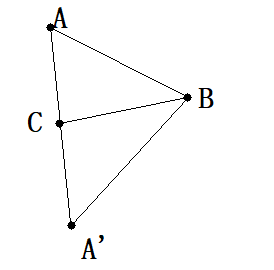
\includegraphics[scale=0.6]{1-3.png}
		\caption{}
		\label{fig:4}
	\end{figure}
	Since $|AC|=|A'C|$, $S_{ABC}=S_{A'BC}$. It means however we move the coins, the area of the triangle is fixed. Therefore, one cannot end up with a bigger triangle. Since in a equilateral triangle, $S=\alpha l^2$ ($\alpha$ is a fixed number and l is the sid length), we cannot ended up with a bigger equilateral triangle.\\
	
	\textbf{Exercise 1.5}\par
	As we have proved in Exercise 1.7 that we cannot form a larger square, of course we cannot form a square of side length 2.\\
	
	
	\textbf{Exercise 1.6}\par
	Include the 4 coins into a rectangular coordinate as the following figure.
	\begin{figure}[H]
		\centering
		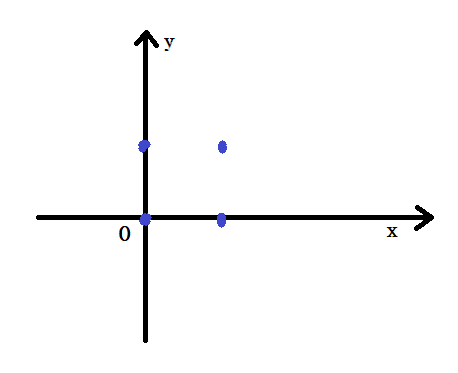
\includegraphics[scale=0.6]{1-6.png}
		\caption{}
		\label{fig:5}
	\end{figure}
	The original coordinates of the 4 coins are (0,0), (0,1), (1,0), (1,1) respectively.
	For any coins locating in $(x_1,y_1)$, after jumping through another coins locating in $(x_2,y_2)$, its new coordinate will be $(2x_2-x_1,2y_2-y_1)$,\  (\ $x_1,y_1,x_2,y_2 \in \mathbb{Z}$\ ).
	In this way, it is clear to conclude that: \\
	$$2x_2-x_1 \equiv x_1\ (mod 2)$$
	$$2y_2-y_1 \equiv y_1\ (mod 2)$$
	Thus, the coin originally locating in (0,0) can only move to: $$(x_1,y_1),x_1,y_1 \in \{x|x=2n,n\in\mathbb{Z}\} $$
	The coin originally locating in (0,1) can only move to: $$(x_2,y_2),x_2\in \{x|x=2n,n\in\mathbb{Z}\}, y_2\in\{x|x=2n+1,n\in\mathbb{Z}\} $$
	The coin originally locating in (1,0) can only move to: $$(x_3,y_3),x_3,\in \{x|x=2n+1,n\in\mathbb{Z}\},y_3\in\{x|x=2n,n\in\mathbb{Z}\} $$
	The coin originally locating in (1,1) can only move to: $$(x_4,y_4),x_4,y_4 \in \{x|x=2n+1,n\in\mathbb{Z}\} $$
	Obviously,you cannot achieve a position in which two coins are at the same position.\\
	
	\textbf{Exercise 1.7}\par
	As we can see from the jumping rule, if coin A jumps to a new place via coin B, we let coin A jumps again via coin B. It is clear that coin A will come back to its original place.\\
	So if we have a method to form a larger square with side length $L$ ($L>1$), then we can form a $1-length$ square from $L-length$ square ($L>1$) by reversing the jumping order. Then we will prove that there is no way to form a $1-length$ square from L-length square ($L>1$).\\
	We design a rectangular coordinate system, and in the beginning, the four coins are at $(0,0) (0,L) (L,0) (L,L)$ respectively. The four $x-coordinates$ and four $y-coordinates$ are all integral multiple of L. In one jump, let's suppose coin A at $(x_1 \cdot L,y_1 \cdot L)$ jumping via coin B at $(x_2 \cdot L,y_2 \cdot L)$, in which $x_1$, $x_2$, $y_1$, $y_2$ are all integers. Then coin A reaches ($(2 x_2-x_1)\cdot L,(2 y_2 - y_1)\cdot L$), which coordinates are also integral multiple of L. So every coin can only exist in coordinates with integral multiple of L. It means that unless some coins are at the same position, the least distance between two coins is $L$ ($L>1$). So we cannot form a $1-length$ square.
	
	
	
	\section{Feasible Intersection Patterns}
	\textbf{Exercise 2.1}\par
	1.We use Venn diagrams to prove it.
	\begin{figure}[H]
		\centering
		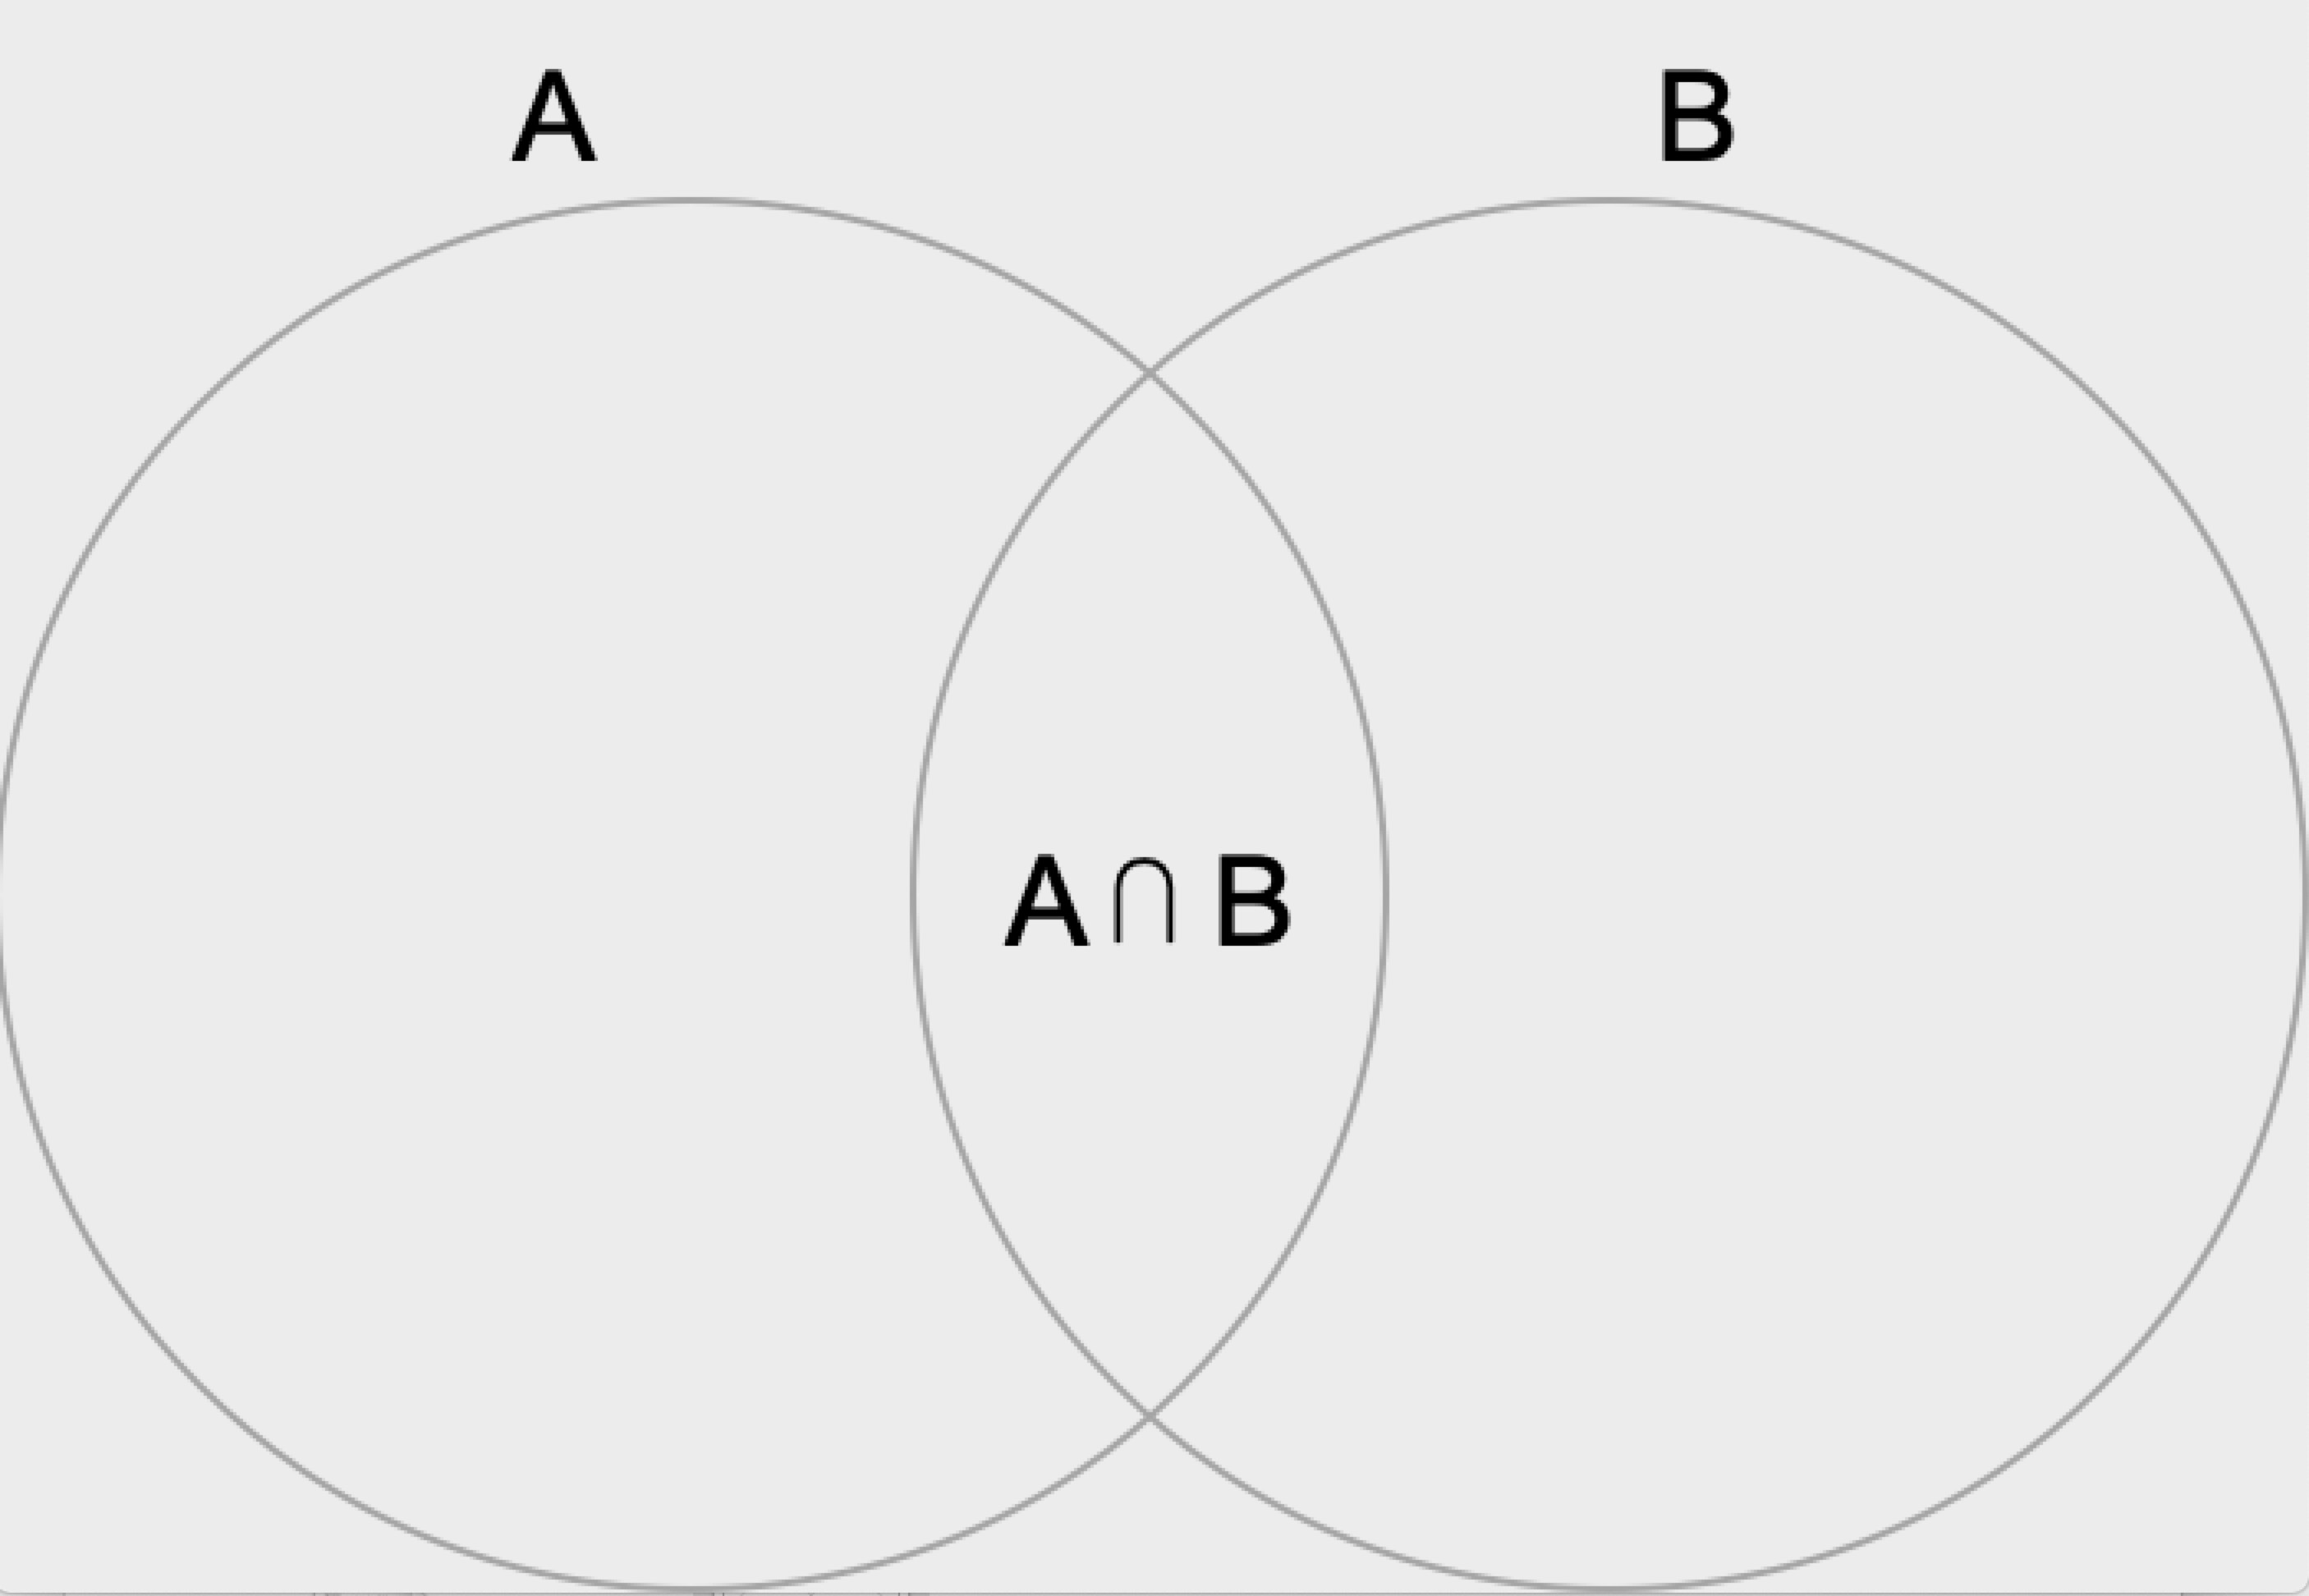
\includegraphics[scale=0.06]{IMG_4576.JPG}
		\caption{}
		\label{fig:6}
	\end{figure}
	From the figure above, we can see $|A\cap B|$ accumulated twice in $|A|+|B|$. We should minus one $|A\cap B|$. Therefore, $|A\cup B|=|A|+|B|-|A\cap B|$.\\
	
	2. Solution. $$|A\cup B\cup C|=|A|+|B|+|C|-|A\cap B|-|A\cap C|-|B\cap C|+|A\cap B\cap C|$$
	
	3. Solution. $$|A\cup B\cup C\cup D|=|A|+|B|+|C|+|D|-|A\cap B|-|A\cap C|-|A\cap D|-|B\cap C|-|B\cap D|-|C\cap D|+|A\cap B\cap C|$$ $$+|A\cap B\cap D|+|A\cap C\cap D|+|B\cap C\cap D|-|A\cap B\cap C\cap D|$$
	
	\textbf{Exercise 2.2}\par
	Let S be finite set $S=\{1,2,3,\cdots ,n\}$\\
	$$|A_1\cup A_2\cup \cdots \cup A_n|=\sum_{I\in 2^S}(-1)^{|I|-1}|A_I|,\ A_I:=\bigcap_{i\in I}A_i$$
	
	
	\textbf{Exercise 2.3}\par
	\textbf{Proof1.} We use induction on n.\\
	1) Basic step. n=2, $|A_1\cup A_2|=|A_1|+|A_2|-|A_1\cap A_2|$. It is justified by Exercise 2.1.1.\\
	2) Induction hypothesis. Assume n=k satisfy the following formula for integer $k\ge2$. Let S be finite set $S=\{1,2,3,\cdots ,k\}$. $$|A_1\cup A_2\cup \cdots \cup A_k|=\sum_{I\in 2^S}(-1)^{|I|-1}|A_I|,\ A_I:=\bigcap_{i\in I}A_i$$\\
	
	3) Proof of induction step. Now let us prove that based on the induction hypothesis of n=k, we can get the same fomula for n=k+1.
	$$|A_1\cup A_2\cup \cdots \cup A_k\cup A_{k+1}|=|A_1\cup A_2\cup \cdots \cup A_k|+|A_{k+1}|-|(A_{k+1}\cap A_1)\cup (A_{k+1}\cap A_2)\cup \cdots \cup(A_{k+1}\cap A_k)|$$
	$$=\sum_{I\in 2^T}(-1)^{|I|-1}|A_I|+|A_{k+1}|-\sum_{I\in 2^T}(-1)^{|I|-1}|A_I\cap A_{k+1}|$$
	$$=\sum_{I\in 2^T}(-1)^{|I|-1}|A_I|,\ A_I:=\bigcap_{i\in I}A_i\ \ T\ is\ finite\ set\ \ T=\{1,2,\cdots ,k+1\}$$
	
	\textbf{Proof2.}We do not use induction. We need to prove that any element in the $A_i$ set is added exactly once by the formula on the right.\\
	We assume there is an arbitrary element x in k sets of $A_i$\\
	When $|I|=1$, element x is added k times.\\
	When $| I | = 2$,element $x$ is reduced $C_k^2$ times.\\
	When $| I | = 3$,element $x$ is added $C_k^3$ times.\\
	\qquad\vdots\\
	\qquad\vdots\\
	When $| I | = k$,element $x$ is added/reduced $C_k^k$ times\\
	and the symbol is determined by $(-1)^{k-1}$.\\
	Then we calculate the sum.\\
	$$Sum = C_k^1 - C_k^2 + C_k^3 - \cdots\cdots + (-1)^{i-1}C_k^i + \cdots\cdots + (-1)^{k-1}C_k^k$$
	According to binonial theorem,we have\\
	$$(1-x)^k = C_k^0 - C_k^1 \cdot x + C_k^2 \cdot x^2 - C_k^3 \cdot x^3 + \cdots + (-1)^k \cdot C_k^k \cdot x^k$$
	We let $x$ be $1$,then we have\\
	$$1 - C_k^1 + C_k^2 - C_k^3 + \cdots -(-1)^{k-1}C_k^k = 0$$
	Therefore,$1 - Sum = 0,Sum = 1$.\\
	\qquad Proof completed.\\
	
	
	
	
	\section{Feasible Intersection Patterns}
	\textbf{Exercise 3.1}\par
	We give the following example:
	$$A_1=\{1,2,3,4,5,6\}$$
	$$A_2=\{4,5,6,7,8,9\}$$
	$$A_3=\{2,3,4,7,8,10\}$$
	$$A_4=\{1,2,5,7,9,10\}$$
	Let's check it.
	$$A_1 \cap A_2=\{4,5,6\}	, A_1 \cap A_3=\{2,3,4\} ,	A_1 \cap A_4=\{1,2,5\}$$
	$$A_2 \cap A_3=\{4,7,8\}	, A_2 \cap A_4=\{5,7,9\} ,	A_3 \cap A_4=\{2,7,10\}$$
	These pairwise intersections all have 3 elements.
	$$A_1 \cap A_2 \cap A_3=\{4\}	, A_1 \cap A_2 \cap A_4=\{5\}$$
	$$A_1 \cap A_3 \cap A_4=\{2\}	, A_2 \cap A_3 \cap A_4=\{7\}$$
	These three-wise intersections all have 1 element.\\
	
	
	\textbf{Exercise 3.2}\par
	We insist that $\mid A_i \mid =5$ for $i=1 ,2,3,4$.\\
	According to The Exclusion-Inclusion Formula, each pairwise union has $5+5-3=7$ elements, \\
	and each three-wise union has $5+5+5-3-3-3+1=7$ elements.\\
	Let's take $A_1$ for example. Obviously, $$A_2 \cup A_3 \subseteq A_1 \cup A_2 \cup A_3$$, and they have the same number of elements,\\
	so $$A_2 \cup A_3 = A1 \cup A_2 \cup A_3$$. Then $$A_1 \subseteq A_2 \cup A_3$$.\\
	Similarly, we can prove that $$A_4 \subseteq A_2 \cup A_3$$.\\
	So $$A_2 \cup A_3=A_1 \cup A_2 \cup A_3 \cup A_4$$, $$A_1 \cup A_2 \cup A_3 \cup A_4$$ also has $7$ elements.\\
	Without s of generality suppose that\\
	$$A_1 \cup A_2 \cup A_3 \cup A_4=\{1,2,3,4,5,6,7\}$$ and $$A_1=\{1,2,3,4,5\}$$
	In order to satisfy the requirement that all pairwise intersections\\
	have size $3$, each of $A2$, $A3$, $A4$ must have only $3$ elements in $\{1,2,3,4,5\}$, \\so they must include $\{6,7\}$ (each set has size $5$).\\
	Then $$\{6,7\} \in A_2 \cup A_3 \cup A_4$$, $$ \mid A_2 \cup A_3 \cup A_4 \mid \ge 2$$, which contradicts the requirement that all three-wise intersections have size $1$.\\
	So if we insist that $$ \mid A_i\mid  = 5$$ for all $i$, then the task of Exercise 3.1 cannot be solved.\\
	
	\textbf{Exercise 3.3}\par
	Suppose sets $A_1,A_2,\cdots,A_n$ satisfy the conditions.\par
	Let$B_I=\bigcap_{i\in I}A_i \backslash (\bigcup_{j\notin I} A_j)$\par
	Let$|B_I|=b_i\ ,\ |I|=i$\par
	It is clear that
	$$B_{I_1}\cap B_{I_2}=\phi\ ,\ I_1\neq I_2$$

	$$A_I=\bigcup B_{I'}\ ,\ I\subseteq I'\subseteq \{1,2,\cdots ,n\}$$

	$$Thus,\ |A_I|=\sum |B_{I'}|=\ ,\ I\subseteq I'\subseteq \{1,2,\cdots ,n\}$$

	$$Thus,\ a_i=C^0_{n-i}b_1+C^1_{n-i}b_2+\cdots +C^{n-i}_{n-i}b_n$$

	$$B_I=A_I\backslash \bigcup A_{I'}\ ,\ I\subsetneqq I'\subseteq \{1,2,\cdots ,n\}$$

	$$Thus,\ b_i=a_i-\sum^n_{k=i+1} C^{k-i}_{n-i}(-1)^{k-i+1}a_k$$

	It is obvious if and only if $\forall b_j\ ,\ j\in \{1,2,\cdots,n\}\ ,\ b_j\geq 0$, the condition can be satisfied.\par

	In another word, $C^0_{n-j}a_j-C^1_{n-j}a_{j+1}+\cdots +(-1)^{n-j+1}C^{n-j}_{n-j}a_n\geq 0$.\par
	
	In conclusion, $$\forall a_j\ (j=1,2,\cdots,n)\ ,\ a_j\geq C^1_{n-j}a_{j+1}-C^2_{n-j}a_{j+2}+\cdots +(-1)^{n-j+1}C^{n-j}_{n-j}a_n$$
	
\end{document}

